%!TEX program = xelatex
% 完整编译: xelatex -> biber/bibtex -> xelatex -> xelatex
\documentclass[lang=cn,a4paper,citestyle=gb7714-2015, bibstyle=gb7714-2015]{elegantpaper}

\title{NSGA-II算法}

\author{姜孟冯 \\中国矿业大学 / 应急管理部信息研究院}

\date{\zhtoday}

%%%%%%%%%%%%%%%%%%%%%%%%%%%%%%%%%%%%%%%%%%%%%%%%%%%%%%%%%%%%%%%%%%%%%
% PACKAGES                                                          %
%%%%%%%%%%%%%%%%%%%%%%%%%%%%%%%%%%%%%%%%%%%%%%%%%%%%%%%%%%%%%%%%%%%%%
\usepackage{amssymb}
\usepackage{optidef}
\usepackage{pgfplots}
\usepackage{tabularray}
\usepackage{biblatex}
\addbibresource[location=local]{reference.bib} % 参考文献
%%%%%%%%%%%%%%%%%%%%%%%%%%%%%%%%%%%%%%%%%%%%%%%%%%%%%%%%%%%%%%%%%%%%%%
% STYLE ENVIRONMENT                                                %
%%%%%%%%%%%%%%%%%%%%%%%%%%%%%%%%%%%%%%%%%%%%%%%%%%%%%%%%%%%%%%%%%%%%%%
\usepgfplotslibrary{fillbetween}
\pgfplotsset{
    my axis style/.style={
        axis lines=middle, % 将坐标轴置于图形中心
        unit vector ratio=1 1 1, % 设置 x 轴和 y 轴的单位长度比例
        %        xmin=0,  % x 轴范围
        %        ymin=0,  % y 轴范围
        axis on top,
        xlabel={$x_1$},
        ylabel={$x_2$},
        legend pos=outer north east,
    }
}

\NewTblrEnviron{simplex}
\SetTblrInner[simplex]{
    cells  = {c, m},
    row{2} = {mode = math},
    column{1,2} = {mode = math},
    hline{1,Z} = {0.15em},
    hline{2,3,Y} = {0.08em},
    vline{4} = {0.08em},
    cell{1}{1} = {c=3,r=1}{c},
    cell{Z}{1} = {c=3,r=1}{c},
}
\UseTblrLibrary{diagbox}

%%%%%%%%%%%%%%%%%%%%%%%%%%%%%%%%%%%%%%%%%%%%%%%%%%%%%%%%%%%%%%%%%%%%%%
% MY COMMANDS                                                        %
%%%%%%%%%%%%%%%%%%%%%%%%%%%%%%%%%%%%%%%%%%%%%%%%%%%%%%%%%%%%%%%%%%%%%%
\newcommand{\R}{\mathbf{R}}
\newcommand{\C}{\mathbf{C}}
\newcommand{\F}{\mathbf{F}}
\newcommand{\U}{\mathit{U}}
\newcommand{\V}{\mathit{V}}
\newcommand{\W}{\mathit{W}}
\newcommand{\poly}{\mathcal{P}}
\newcommand{\espace}{\mathcal{L}}
\newcommand{\expect}{\mathcal{E}}
\newcommand{\mat}{\mathcal{M}}
\newcommand{\mtxA}{\mathcal{A}}
\DeclareMathOperator{\Span}{span}
\DeclareMathOperator{\Real}{Re}
\DeclareMathOperator{\Imag}{Im}
\DeclareMathOperator{\Null}{null}
\DeclareMathOperator{\Range}{range}
\newcommand{\ph}{\phantom{+x_0}}
%\newcommand{\bigO}{\mathcal{O}}
%\newcommand{\mat}{\mathcal{M}}
%\newcommand{\defeq}{\vcentcolon=}
%\newcommand{\restr}[1]{|_{#1}}

%%%%%%%%%%%%%%%%%%%%%%%%%%%%%%%%%%%%%%%%%%%%%%%%%%%%%%%%%%%%%%%%%%%%%%
% SECTION SETTINGS                                               %
%%%%%%%%%%%%%%%%%%%%%%%%%%%%%%%%%%%%%%%%%%%%%%%%%%%%%%%%%%%%%%%%%%%%%%
%\renewcommand{\thesubsection}{\thesection\Alph{subsection}}
%\renewcommand{\thesubsubsection}{\arabic{subsubsection}}

%%%%%%%%%%%%%%%%%%%%%%%%%%%%%%%%%%%%%%%%%%%%%%%%%%%%%%%%%%%%%%%%%%%%%%
% DOCUMENT                                                           %
%%%%%%%%%%%%%%%%%%%%%%%%%%%%%%%%%%%%%%%%%%%%%%%%%%%%%%%%%%%%%%%%%%%%%%
\begin{document}

    \maketitle

    \section{算法背景}
    \subsection{多目标优化问题}
    \textbf{多目标优化问题(MOP)}是涉及多个目标函数同时优化的数学问题。
    需要在两个或多个相互冲突的目标之间进行权衡的情况下作出最优决策。

    \begin{definition}
        多目标优化问题(multi-objective optimization problem,简称MOP)
        \begin{mini*}|s|
            {}
            {F(X) = (f_1(X),f_2(X), \dots , f_r(X))}
            {}
            {}
            \addConstraint{g_i(X)}{\geq 0,i=1,2,\dots,k}
            \addConstraint{h_i(X)}{= 0,i=1,2,\dots,l}
        \end{mini*}
        记该问题的可行解集为
        $$\Omega = \{X\in \R^n|g_i(X)\geq0,h_j(X)=0 (i=1,2,\dots,k,j=1,2,\dots,l)\}$$
    \end{definition}

    \begin{definition}
        Pareto支配(Pareto Dominance)\\
        X支配Y,记为 $X \prec Y$ ,当且仅当以下条件同时成立
        $$\forall{i}\in\{1,2,\dots,r\}, f_i(X) \leq f_i(Y)\ \ \text{且}\ \ \exists {j} \in \{1,2,...,r\}, f_j(X)<f_j(Y)$$
    \end{definition}


    \begin{definition}
        Pareto最优解集(Pareto Optimal Set)\\
        如果一个可行解$X^*\in \Omega$被称之为Pareto optimal solution, 当且仅当 $X^∗$ 不被其他的解支配。易见$X^*$往往不是一个,常常用$\{X^*\}$表示最优解集
        $$P^*=\{X^*\}=\{X\in\Omega|\neg\exists X'\in\Omega,f_j(X')\leq f_j(X) (j=1,2,\dots,r)\} $$
    \end{definition}

    \begin{definition}
        Pareto边界(Pareto Front,简称PF)\\
        Pareto Optimal Set 中每个解对应的目标值向量组成的集合称之为Pareto Front。
        $$PF^*=\{f(X) = (f_1(X),f_2(X), \dots, f_r(X))|X\in\{X^*\}\}$$
    \end{definition}

    值得注意的是,Pareto最优解集是决策向量空间的一个子集$P^*\subseteq\Omega\subseteq\R^n$,而Pareto边界是目标向量空间的一个子集$PF^*\subseteq\varPi\subseteq\R^r$.

%        \begin{figure}[H]
%              \centering
%              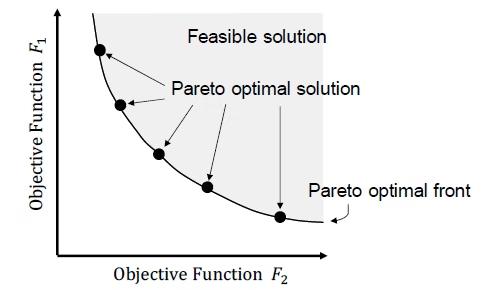
\includegraphics{ParetoFront.avif}
%              \caption{Pareto边界示意图}
%            \end{figure}

    \subsection{多目标进化算法与分类}
    \textbf{多目标进化算法(Multi-objective Evolutionary Algorithm,简称MOEA)}是一种非常有效的解决多目标优化问题(MOP)的方法。1989年,David Goldberg在其著作《Genetic Algorithm in Search, Optimization and Machine Learning\parencite{goldberg1989genetic}》中,提出了用进化算法实现多目标的优化技术,对多目标进化算法的研究具有重要的方向性指导意义。

    根据不同的进化机制,MOEA可以分为三类:
    \begin{enumerate}
        \item 基于分解的MOEA:权重聚合函数、切比雪夫聚合、基于惩罚的边界交叉、MOEA/D
        \item 基于支配关系的MOEA:NSGA-II、NPGA、SPEA2、PESA、PAES、MOMGA、mBOA、MMOGA
        \item 基于指标的MOEA:SMS-EMOA、IBEA、HypE
    \end{enumerate}

    \subsection{NSGA-II算法}
    1994年,Srinivas和Deb提出了NSGA(nondominated sorting in genetic algorithm)\parencite{NSGA},可以有效求解MOP问题,但仍存在一些不足之处:(1)缺少最优个体保留机制(2)共享参数大小不易确定(3)构造非支配集的时间复杂度高$(O(rN^3))$。2000年,Deb等对算法进行优化,提出了NSGA-II\parencite{NSGA2prototype},2002年又对其中的非支配集排序方法进行了改进\parencite{NSGA2},把时间复杂度提高到$(O(rN^2))$,但只适用于处理低维优化问题(维数小于等于3)。2013年,Deb等又提出了NSGA-III(the reference-point based many-objective NSGA-II),用以解决高维数问题。\\

    本文主要集中讨论NSGA-II算法。

    \section{NSGA-II算法原理及框架}
    \subsection{算法框架}
    NSGA-II算法是一种多目标进化算法,全称是Elitist Non-dominated Sorting Genetic Algorithm(精英非支配排序遗传算法),NSGA-II的主要特征有三点:
    \begin{itemize}
        \item 基于高速非支配排序的排序方法
        \item 基于拥挤度的比较方法
        \item 通过二进制锦标赛机制进行遗传操作
    \end{itemize}

    NSGA-II算法基于遗传算法的逐代进化思想,使用非支配排序和拥挤度计算来分配适应度。非支配排序将个体分为不同的等级,等级越低,个体的适应度越高。拥挤度计算则衡量个体在目标空间中的拥挤程度,拥挤度越低,个体的适应度越高。

    其基本框架如下:
    %        \begin{figure}[H]
        %              \centering
        %              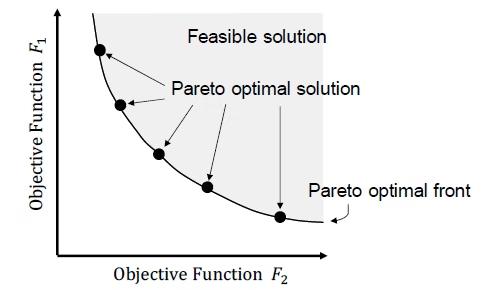
\includegraphics{ParetoFront.avif}
        %              \caption{Pareto边界示意图}
        %            \end{figure}

    \subsection{非支配集排序方法}


    \subsection{拥挤度计算方法}
    拥挤度可以使用聚集距离来评价,设下标为i的个体的拥挤度记为$d_i$,目标函数值记为$f_k(x_i)$,用$f_k^{max}$与$f_k^{min}$分别表示目标函数的最大最小值,则拥挤度计算可使用以下公式:
    $$d_i = \sum_{k=1}^M(\dfrac{f_k(x_{i+1}) - f_k(x_{i-1})}{f_k^{max} - f_k^{min}})$$


    \subsection{选择机制}
    NSGA-II算法使用二进制锦标赛选择机制。在每次选择中,算法从种群中随机选择两个个体,并根据它们的非支配等级和拥挤度进行比较。适应度较高的个体将被选中。

    \section{算法步骤及实现}
    \subsection{参数设置}
    NSGA-II算法的参数设置对算法的性能有重要影响。主要参数包括:

    **种群规模(N):**控制种群中个体的数量。较大的种群规模可以提供更广泛的搜索空间,但计算成本更高。
    **最大进化代数(MaxGen):**控制算法运行的代数。较大的最大进化代数可以提高算法的收敛性,但计算成本也更高。
    **交叉概率(Pc):**控制交叉算子应用的概率。较高的交叉概率可以促进种群多样性,但可能导致过早收敛。
    **变异概率(Pm):**控制变异算子应用的概率。较高的变异概率可以引入新的个体,但可能破坏种群的收敛性。

    \subsection{基本步骤}

    NSGA-II算法的实现步骤如下:

    **初始化种群:**随机生成一个N个个体的初始种群。
    **评估种群:**计算每个个体的目标函数值和约束条件值。
    **非支配排序:**将种群中的个体根据非支配关系进行排序。
    **拥挤度计算:**计算每个个体的拥挤度,衡量个体在目标空间中的密度。
    **选择:**根据非支配等级和拥挤度,选择下一代的个体。
    **交叉:**对选定的个体进行交叉操作,产生新的个体。
    **变异:**对新的个体进行变异操作,引入新的基因。
    **合并:**将新的个体与当前种群合并,形成新的种群。
    **重复步骤2-8:**重复上述步骤,直到达到最大进化代数或满足终止条件。
    (1)随机初始化开始种群$P_0$ ,数量为n。并对$P_0$进行非支配排序,初始化每个个体的rank值;
    (2)t = 0;
    (3)通过选择操作从Pt选择个体,并进行交叉和变异操作,产生新一代种群Qt;
    (4)通过合并Pt 和 Qt 产生出组合种群Rt =  Pt UQt ;
    (5)对Rt进行非支配排序,并选出n个个体,组成新一代种群Pt+1;
    (6)跳转到步骤3,并循环,直至满足结束条件。

    \subsection{开源算法实现}

    \begin{enumerate}
        \item java:MOEA Framework:https://github.com/MOEAFramework/MOEAFramework
        \item 基于分解的方法:MOEA/D
        \item 基于indicator的方法:IBEA、HypE
    \end{enumerate}

    \section{算法应用}
    NSGA-II算法应用非常广泛,

    \subsection{工程设计优化}

    工程设计优化是NSGA-II算法最常见的应用领域之一。在工程设计中,往往需要同时考虑多个目标,如成本、性能、可靠性等。NSGA-II算法可以有效地处理多目标优化问题,找到满足所有目标约束的最佳解决方案。

    案例:飞机机翼设计优化

    飞机机翼设计是一个典型的多目标优化问题,需要同时考虑机翼的升力、阻力、重量等多个目标。使用NSGA-II算法对飞机机翼进行优化,可以找到满足升力、阻力、重量约束的最佳机翼形状。
    逻辑分析:

    定义目标函数:计算飞机机翼的升力和阻力。
    定义NSGA-II算法:包含初始化种群、迭代优化、选择操作、交叉和变异操作等步骤。
    拥挤度计算:计算种群中个体的拥挤度,用于选择操作。
    交叉操作:对两个父个体进行交叉,生成两个子个体。
    变异操作:对个体进行变异,引入多样性。
    运行NSGA-II算法:迭代优化,找到最优解。
    输出最优解:打印飞机机翼的最佳形状。

    \subsection{资源分配优化}

    资源分配优化是NSGA-II算法的另一个重要应用领域。在资源分配问题中,需要在有限的资源约束下,将资源分配给多个任务或项目,以最大化整体收益或最小化成本。NSGA-II算法可以有效地解决此类问题,找到满足资源约束的最佳分配方案。

    案例:项目组合优化

    项目组合优化是一个典型的资源分配优化问题,需要在有限的预算约束下,选择一组项目进行投资,以最大化投资回报率。使用NSGA-II算法对项目组合进行优化,可以找到满足预算约束的最佳项目组合。

    NSGA-II算法在风力发电机组优化中得到了广泛的应用。风力发电机组优化涉及到多目标,如发电量最大化、成本最小化和环境影响最小化。

    应用步骤:

    定义目标函数:
    %
    %发电量:P = 0.5 * ρ * A * V^3 * C_p
    %成本:C = C_i + C_o * P
    %环境影响:E = N_b * P
    %其中,ρ为空气密度,A为叶片面积,V为风速,C_p为功率系数,C_i为初始成本,C_o为运行成本,N_b为噪声水平。

    \subsection{数据挖掘优化}
    数据挖掘优化是NSGA-II算法的又一应用领域。在数据挖掘中,需要从大量数据中提取有价值的信息,如模式、规则或分类器。NSGA-II算法可以优化数据挖掘算法的参数,以提高挖掘效率和准确性。

    案例:特征选择优化

    特征选择是数据挖掘中的一个重要步骤,需要从原始数据集中选择最具区分性的特征。使用NSGA-II算法对特征选择进行优化,可以找到满足分类或回归任务要求的最佳特征子集。


    \nocite{*}
    \printbibliography[heading=bibintoc, title=\ebibname]
\end{document}
